\pdfoutput=1

%\documentclass[preprint,10pt]{elsarticle}
%\documentclass[preprint,10pt]{amsart}
\documentclass[review]{siamart0216}
%\documentclass{siamart0216}

%\usepackage{fullpage}
%\usepackage[colorlinks=true]{hyperref}

\usepackage{amsmath,amssymb,amsfonts}
%\usepackage{amsthm}
%\theoremstyle{definition}
%\newtheorem{definition}{Definition}
%\theoremstyle{lemma}
%\newtheorem{lemma}{Lemma}
%\theoremstyle{corollary}
%\newtheorem{corollary}{Corollary}
%\newtheorem*{remark}{Remark}
%\theoremstyle{theorem}
%\newtheorem{theorem}{Theorem}
%\theoremstyle{assumption}
%\newtheorem{assumption}{Assumption}

\usepackage[titletoc,toc,title]{appendix}

\usepackage{array} 
\usepackage{listings}
\usepackage{mathtools}
\usepackage{pdfpages}
\usepackage[textsize=footnotesize,color=green]{todonotes}
\usepackage{bm}
\usepackage{bbm}

\usepackage{tikz}
\usepackage[normalem]{ulem}
\usepackage{hhline}

\usepackage{graphicx}
\usepackage{subfig}
\usepackage{color}

%% ====================================== graphics

\usepackage{pgfplots}
\usepackage{pgfplotstable}
\definecolor{markercolor}{RGB}{124.9, 255, 160.65}
\pgfplotsset{
compat=1.3,
width=10cm,
tick label style={font=\small},
label style={font=\small},
legend style={font=\small}
}

\usetikzlibrary{calc}
\usetikzlibrary{intersections} 

%%% START MACRO FOR ANNOTATION OF TRIANGLE WITH SLOPE %%%.
\newcommand{\logLogSlopeTriangle}[5]
{
    % #1. Relative offset in x direction.
    % #2. Width in x direction, so xA-xB.
    % #3. Relative offset in y direction.
    % #4. Slope d(y)/d(log10(x)).
    % #5. Plot options.

    \pgfplotsextra
    {
        \pgfkeysgetvalue{/pgfplots/xmin}{\xmin}
        \pgfkeysgetvalue{/pgfplots/xmax}{\xmax}
        \pgfkeysgetvalue{/pgfplots/ymin}{\ymin}
        \pgfkeysgetvalue{/pgfplots/ymax}{\ymax}

        % Calculate auxilliary quantities, in relative sense.
        \pgfmathsetmacro{\xArel}{#1}
        \pgfmathsetmacro{\yArel}{#3}
        \pgfmathsetmacro{\xBrel}{#1-#2}
        \pgfmathsetmacro{\yBrel}{\yArel}
        \pgfmathsetmacro{\xCrel}{\xArel}

        \pgfmathsetmacro{\lnxB}{\xmin*(1-(#1-#2))+\xmax*(#1-#2)} % in [xmin,xmax].
        \pgfmathsetmacro{\lnxA}{\xmin*(1-#1)+\xmax*#1} % in [xmin,xmax].
        \pgfmathsetmacro{\lnyA}{\ymin*(1-#3)+\ymax*#3} % in [ymin,ymax].
        \pgfmathsetmacro{\lnyC}{\lnyA+#4*(\lnxA-\lnxB)}
        \pgfmathsetmacro{\yCrel}{\lnyC-\ymin)/(\ymax-\ymin)} % THE IMPROVED EXPRESSION WITHOUT 'DIMENSION TOO LARGE' ERROR.

        % Define coordinates for \draw. MIND THE 'rel axis cs' as opposed to the 'axis cs'.
        \coordinate (A) at (rel axis cs:\xArel,\yArel);
        \coordinate (B) at (rel axis cs:\xBrel,\yBrel);
        \coordinate (C) at (rel axis cs:\xCrel,\yCrel);

        % Draw slope triangle.
        \draw[#5]   (A)-- node[pos=0.5,anchor=north] {}
                    (B)-- 
                    (C)-- node[pos=0.5,anchor=west] {\textcolor{black}{#4}}
                    cycle;
    }
}
%%% END MACRO FOR ANNOTATION OF TRIANGLE WITH SLOPE %%%.

\newcommand{\logLogSlopeTriangleNeg}[5]
{
    % #1. Relative offset in x direction.
    % #2. Width in x direction, so xA-xB.
    % #3. Relative offset in y direction.
    % #4. Slope d(y)/d(log10(x)).
    % #5. Plot options.

    \pgfplotsextra
    {
        \pgfkeysgetvalue{/pgfplots/xmin}{\xmin}
        \pgfkeysgetvalue{/pgfplots/xmax}{\xmax}
        \pgfkeysgetvalue{/pgfplots/ymin}{\ymin}
        \pgfkeysgetvalue{/pgfplots/ymax}{\ymax}

        % Calculate auxilliary quantities, in relative sense.
        \pgfmathsetmacro{\xArel}{#1}
        \pgfmathsetmacro{\yArel}{#3}
        \pgfmathsetmacro{\xBrel}{#1-#2}
        \pgfmathsetmacro{\yBrel}{\yArel}
        \pgfmathsetmacro{\xCrel}{\xArel}

        \pgfmathsetmacro{\lnxB}{\xmin*(1-(#1-#2))+\xmax*(#1-#2)} % in [xmin,xmax].
        \pgfmathsetmacro{\lnxA}{\xmin*(1-#1)+\xmax*#1} % in [xmin,xmax].
        \pgfmathsetmacro{\lnyA}{\ymin*(1-#3)+\ymax*#3} % in [ymin,ymax].
        \pgfmathsetmacro{\lnyC}{\lnyA+#4*(\lnxA-\lnxB)}
        \pgfmathsetmacro{\yCrel}{\lnyC-\ymin)/(\ymax-\ymin)} % THE IMPROVED EXPRESSION WITHOUT 'DIMENSION TOO LARGE' ERROR.

        % Define coordinates for \draw. MIND THE 'rel axis cs' as opposed to the 'axis cs'.
        \coordinate (A) at (rel axis cs:\xArel,\yArel);
        \coordinate (B) at (rel axis cs:\xBrel,\yBrel);
        \coordinate (C) at (rel axis cs:\xCrel,\yCrel);

        % Draw slope triangle.
        \draw[#5]   (A)-- node[pos=.5,anchor=south] {}
                    (B)-- 
                    (C)-- node[pos=0.5,anchor=west] {\textcolor{black}{#4}}
                    cycle;
    }
}
%%% END MACRO FOR ANNOTATION OF TRIANGLE WITH SLOPE %%%.

%%% START MACRO FOR ANNOTATION OF TRIANGLE WITH SLOPE %%%.
\newcommand{\logLogSlopeTriangleFlipNeg}[5]
{
    % #1. Relative offset in x direction.
    % #2. Width in x direction, so xA-xB.
    % #3. Relative offset in y direction.
    % #4. Slope d(y)/d(log10(x)).
    % #5. Plot options.

    \pgfplotsextra
    {
        \pgfkeysgetvalue{/pgfplots/xmin}{\xmin}
        \pgfkeysgetvalue{/pgfplots/xmax}{\xmax}
        \pgfkeysgetvalue{/pgfplots/ymin}{\ymin}
        \pgfkeysgetvalue{/pgfplots/ymax}{\ymax}

        % Calculate auxilliary quantities, in relative sense.
        %\pgfmathsetmacro{\xArel}{#1}
        %\pgfmathsetmacro{\yArel}{#3}
        \pgfmathsetmacro{\xBrel}{#1-#2}
        \pgfmathsetmacro{\yBrel}{#3}
        \pgfmathsetmacro{\xCrel}{#1}

        \pgfmathsetmacro{\lnxB}{\xmin*(1-(#1-#2))+\xmax*(#1-#2)} % in [xmin,xmax].
        \pgfmathsetmacro{\lnxA}{\xmin*(1-#1)+\xmax*#1} % in [xmin,xmax].
        \pgfmathsetmacro{\lnyA}{\ymin*(1-#3)+\ymax*#3} % in [ymin,ymax].
        \pgfmathsetmacro{\lnyC}{\lnyA+#4*(\lnxA-\lnxB)}
        \pgfmathsetmacro{\yCrel}{\lnyC-\ymin)/(\ymax-\ymin)} % THE IMPROVED EXPRESSION WITHOUT 'DIMENSION TOO LARGE' ERROR.

	\pgfmathsetmacro{\xArel}{\xBrel}
        \pgfmathsetmacro{\yArel}{\yCrel}

        % Define coordinates for \draw. MIND THE 'rel axis cs' as opposed to the 'axis cs'.
        \coordinate (A) at (rel axis cs:\xArel,\yArel);
        \coordinate (B) at (rel axis cs:\xBrel,\yBrel);
        \coordinate (C) at (rel axis cs:\xCrel,\yCrel);

        % Draw slope triangle.
        \draw[#5]   (A)-- node[pos=0.5,anchor=east] {\textcolor{black}{#4}}
                    (B)-- 
                    (C)-- node[pos=0.5,anchor=north] {1}
                    cycle;
    }
}
%%% END MACRO FOR ANNOTATION OF TRIANGLE WITH SLOPE %%%.


%%% START MACRO FOR ANNOTATION OF TRIANGLE WITH SLOPE %%%.
\newcommand{\logLogSlopeTriangleFlip}[5]
{
    % #1. Relative offset in x direction.
    % #2. Width in x direction, so xA-xB.
    % #3. Relative offset in y direction.
    % #4. Slope d(y)/d(log10(x)).
    % #5. Plot options.

    \pgfplotsextra
    {
        \pgfkeysgetvalue{/pgfplots/xmin}{\xmin}
        \pgfkeysgetvalue{/pgfplots/xmax}{\xmax}
        \pgfkeysgetvalue{/pgfplots/ymin}{\ymin}
        \pgfkeysgetvalue{/pgfplots/ymax}{\ymax}

        % Calculate auxilliary quantities, in relative sense.
        %\pgfmathsetmacro{\xArel}{#1}
        %\pgfmathsetmacro{\yArel}{#3}
        \pgfmathsetmacro{\xBrel}{#1-#2}
        \pgfmathsetmacro{\yBrel}{#3}
        \pgfmathsetmacro{\xCrel}{#1}

        \pgfmathsetmacro{\lnxB}{\xmin*(1-(#1-#2))+\xmax*(#1-#2)} % in [xmin,xmax].
        \pgfmathsetmacro{\lnxA}{\xmin*(1-#1)+\xmax*#1} % in [xmin,xmax].
        \pgfmathsetmacro{\lnyA}{\ymin*(1-#3)+\ymax*#3} % in [ymin,ymax].
        \pgfmathsetmacro{\lnyC}{\lnyA+#4*(\lnxA-\lnxB)}
        \pgfmathsetmacro{\yCrel}{\lnyC-\ymin)/(\ymax-\ymin)} % THE IMPROVED EXPRESSION WITHOUT 'DIMENSION TOO LARGE' ERROR.

	\pgfmathsetmacro{\xArel}{\xBrel}
        \pgfmathsetmacro{\yArel}{\yCrel}

        % Define coordinates for \draw. MIND THE 'rel axis cs' as opposed to the 'axis cs'.
        \coordinate (A) at (rel axis cs:\xArel,\yArel);
        \coordinate (B) at (rel axis cs:\xBrel,\yBrel);
        \coordinate (C) at (rel axis cs:\xCrel,\yCrel);

        % Draw slope triangle.
        \draw[#5]   (A)-- node[pos=0.5,anchor=east] {\textcolor{black}{#4}}
                    (B)-- 
                    (C)-- node[pos=0.5,anchor=south] {}
                    cycle;
    }
}
%%% END MACRO FOR ANNOTATION OF TRIANGLE WITH SLOPE %%%.



\usepackage{stmaryrd}

\renewcommand{\tilde}{\widetilde}
\renewcommand{\hat}{\widehat}
\renewcommand{\topfraction}{0.85}
\renewcommand{\textfraction}{0.1}
\renewcommand{\floatpagefraction}{0.75}

\newcommand{\vect}[1]{\ensuremath\boldsymbol{#1}}
\newcommand{\tensor}[1]{\underline{\bm{#1}}}
\newcommand{\del}{\triangle}
\newcommand{\curl}{\grad \times}
\renewcommand{\div}{\grad \cdot}

\newcommand{\bbm}[1]{\mathbbm{#1}}
\newcommand{\bs}[1]{\boldsymbol{#1}}
\newcommand{\equaldef}{\stackrel{\mathrm{def}}{=}}

\newcommand{\td}[2]{\frac{{\rm d}#1}{{\rm d}{\rm #2}}}
\newcommand{\pd}[2]{\frac{\partial#1}{\partial#2}}
\newcommand{\nor}[1]{\left\| #1 \right\|}
\newcommand{\LRp}[1]{\left( #1 \right)}
\newcommand{\LRs}[1]{\left[ #1 \right]}
\newcommand{\LRa}[1]{\left\langle #1 \right\rangle}
\newcommand{\LRb}[1]{\left| #1 \right|}
\newcommand{\LRc}[1]{\left\{ #1 \right\}}
\newcommand{\LRceil}[1]{\left\lceil #1 \right\rceil}
\newcommand{\LRl}[1]{\left. #1 \right|}
\newcommand{\pdd}[2]{\frac{\partial^2#1}{\partial#2^2}}
\newcommand{\pdn}[3]{\frac{\partial^{#3}#1}{\partial#2^{#3}}}
\newcommand{\mb}[1]{\mathbf{#1}}
\newcommand{\mbb}[1]{\mathbb{#1}}
\newcommand{\mc}[1]{\mathcal{#1}}
\newcommand{\snor}[1]{\left| #1 \right|}


%\newcommand{\cond}[1]{\kappa\LRp{#1}}
\newcommand{\cond}[2]{\nor{#1}_{#2}\nor{{#1}^{-1}}_{#2}}


\newcommand{\Grad} {\ensuremath{\nabla}}
\newcommand{\Div} {\ensuremath{\nabla\cdot}}
\newcommand{\jump}[1] {\ensuremath{\llbracket#1\rrbracket}}
\newcommand{\avg}[1] {\ensuremath{\LRc{\!\{#1\}\!}}}

\newcommand{\Oh}{{\Omega_h}}
\renewcommand{\L}{L^2\LRp{\Omega}}
\newcommand{\LK}{L^2\LRp{D^k}}
\newcommand{\LdK}{L^2\LRp{\partial D^k}}
\newcommand{\Dhat}{\widehat{D}}
\newcommand{\Lhat}{L^2\LRp{\Dhat}}

\newcommand{\eval}[2][\right]{\relax
  \ifx#1\right\relax \left.\fi#2#1\rvert}

\def\etal{{\it et al.~}}


\newcommand{\note}[1]{{\color{blue}{#1}}}
%\newcommand{\noteOne}[1]{{\color{blue}{#1}}}
%\newcommand{\noteTwo}[1]{{\color{red}{#1}}}
%\newcommand{\note}[1]{#1}
%\newcommand{\noteOne}[1]{#1}
%\newcommand{\noteTwo}[1]{#1}


\newcommand{\LinfDk}{L^{\infty}\LRp{D^k}}

\newcommand{\diag}[1]{{\rm diag}\LRp{#1}}

\newcommand{\Ksub}{K_{\rm sub}}

\newcolumntype{C}[1]{>{\centering\let\newline\\\arraybackslash\hspace{0pt}}m{#1}}

%% d in integrand
\newcommand*\diff[1]{\mathop{}\!{\mathrm{d}#1}}

\makeatletter
\renewcommand\d[1]{\mspace{6mu}\mathrm{d}#1\@ifnextchar\d{\mspace{-3mu}}{}}
\makeatother

%\date{}
\author{Jesse Chan, David C.\ Del Rey Fernandez}
\title{Entropy stable skew-symmetric discontinuous Galerkin formulations on non-conforming meshes}
\graphicspath{{./figs/}}


\begin{document}

\maketitle

%\begin{frontmatter}
%\title{Skew-symmetric formulations for entropy stable discontinuous Galerkin methods on non-conforming meshes}
%
%\author[rice]{Jesse Chan\corref{cor1}}
%\ead{Jesse.Chan@caam.rice.edu}
%\address[rice]{Department of Computational and Applied Mathematics, Rice University, 6100 Main St, Houston, TX, 77005}
%
%\begin{abstract}
%Entropy stable high order methods for nonlinear conservation laws satisfy an inherent discrete entropy inequality.  
%\end{abstract}
%\end{frontmatter}

%\tableofcontents

\section{Introduction}

\section{Entropy stable Gauss-Legendre collocation methods}

\note{Idea: decoupled SBP operators allow for the construction of entropy stable schemes by chaining together different sets of nodes through extrapolation (interpolation) operators.  }

\section{Gauss-Legendre collocation on non-conforming meshes}

On conforming meshes, it is most efficient to utilize both Gauss quadrature for volume integrals and Gauss quadrature for face or surface integrals.  For solutions represented in terms of their values at tensor product volume Gauss nodes, extrapolation to face Gauss nodes can be done in an efficient line-by-line manner using one-dimensional interpolation matrices.  

For non-conforming meshes, it can be advantageous to use composite Gauss quadratures on non-conforming interfaces.  \note{Reference JK and LCW's paper on full-side vs split side mortars.}  However, interpolating the solution at volume Gauss nodes to split-side Gauss nodes is no longer a one-dimensional operation.

\begin{figure}
\centering
\begingroup
\captionsetup{width=.25\linewidth}
\subfloat[Conforming faces]{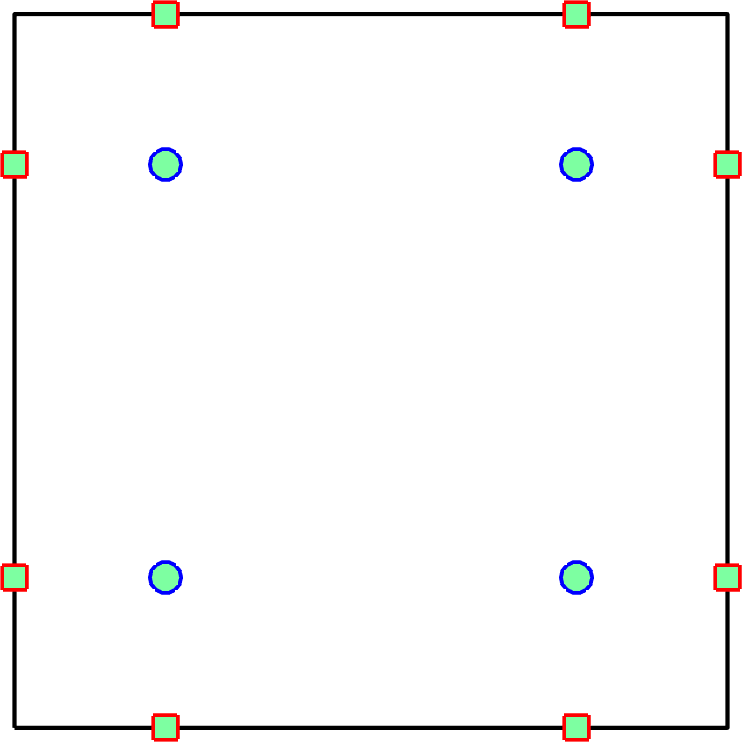
\includegraphics[width=.25\textwidth]{figs/gauss1.png}}
\hspace{4em}
\subfloat[Non-conforming faces]{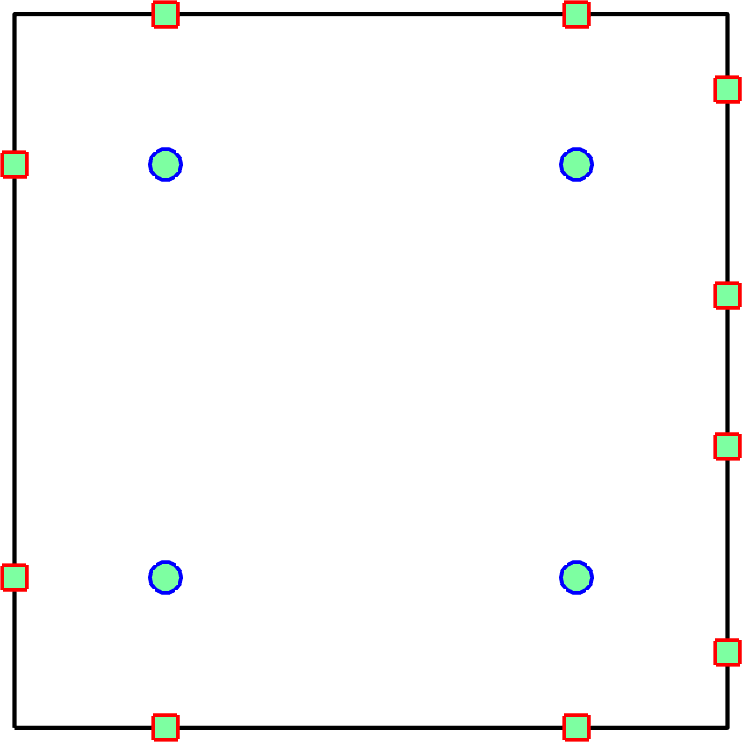
\includegraphics[width=.25\textwidth]{figs/gauss2.png}}
\endgroup
\caption{Examples of surface quadratures for conforming and non-conforming interfaces for Gauss collocation methods.  }
\label{fig:gqcon_noncon}
\end{figure}

It is possible to efficiently interpolate from volume Gauss nodes to split-side Gauss nodes in two steps.  We first interpolate to full-side Gauss nodes on the face, then interpolate from full-side  to split-side Gauss nodes.  Each of these two operations can be done using only one-dimensional interpolation matrices, implying that the interpolation matrix from volume to split-side Gauss nodes can be decomposed into 
\[
\bm{V}_{\rm vol-to-split} = \bm{V}_{\rm vol-to-full} \bm{V}_{\rm full-to-split}
\]
where each of the matrices in the decomposition possess either a sparse or Kronecker product structure.  

ESDG schemes based on decoupled SBP operators introduced in \cite{chan2017discretely} assume a single interpolation matrix which extrapolates from volume to surface nodes.  These schemes require dyadic flux evaluations between all volume and surface nodes connected by this interpolation matrix.  For non-conforming interfaces with split-side Gauss nodes on the face, this necessitates dyadic flux computations between all volume nodes and all split-side Gauss nodes.  

We show in this section how to construct an entropy stable Gauss collocation scheme based on two layers of surface nodes: full-side and split-side nodes.  These surface nodes will be loosely through a skew-symmetric coupling term involving polynomial interpolation matrices between full-side and split-side nodes.  This scheme requires dyadic flux computations between volume and full-side surface nodes, and between full-side and split-side surface nodes.  Each set of dyadic flux computations can be reduced to 

Let ${\bm{V}_f}\tilde{P}_f$ denote the matrix which projects to the trace space using split-side quadrature and evaluates at full-side quadrature points.  Similarly, let $\tilde{\bm{V}_f}{P}_f$ denote the matrix which projects to the trace space using full-side quadrature and evaluates at split-side quadrature points
\begin{align*}
\bm{C}^i_f &= \begin{pmatrix}
\bm{0} & {\rm diag}\LRp{\hat{\bm{n}}_i}{\bm{V}_f}\tilde{\bm{P}}_f\\
-\tilde{\bm{V}_f}{\bm{P}}_f{\rm diag}\LRp{\hat{\bm{n}}_i} &\bm{0}
\end{pmatrix}, \\
\bm{S}^i_f &= \begin{pmatrix}
\diag{\bm{w}_f} & \\
& \diag{\tilde{\bm{w}}_f}
\end{pmatrix}\bm{C}^i_f.
\end{align*}
It is straightforward to show that the matrix $\bm{S}_f$ is skew-symmetric.

%{fig:gqcon_noncon}
Let $\tilde{\bm{F}}_S$ denote the flux matrix, then 
\[
\begin{bmatrix}\bm{L}_f & \tilde{\bm{L}}_f\end{bmatrix} \LRp{\bm{C}^i_f\circ\tilde{\bm{F}}_S}\bm{1}
\]
is a skew-symmetric correction term which ensures entropy stability and high order accuracy (through consistency up to quadrature order).   

Since the difference is high order accurate, you can remove this correction term and still get high order accuracy.  However, the spatial entropy RHS is no longer zero if you use inconsistent surface and coupling quadrature without the correction term (\note{prove this}). 

\note{Do we need 3 layers of surface nodes in 3D?  Interpolation to isotropic split-side nodes is a Kronecker product - does that reduce things down?  }


\bibliographystyle{unsrt}
\bibliography{dg}


\end{document}


